% !TeX root = Protokoll.tex

In den folgenden Abschnitten werden die aufgenommenen Messwerte für jeder der
aufgebauten Schaltungen einzeln ausgewertet. Aufgrund von nicht lösbaren 
Problemen bei der Durchführung des Versuchs wurden uns nach drei Versuchstagen 
die Logarithmierer-/Exponetialgeneratorschaltung  und die Schaltung zur Erzeugung
der gedämpften Sinusspannung  erlassen.

\subsection{Gegengekoppelter Verstärker}

Für die vier Schaltungen eines gegengekoppelten Verstärkers, die 
in diesem Versuchsteil aufgebaut wurden, wurden die Widerstandspaare 
$R_{N}$ und  $R_{1}$ in \cref{tab:gegengekoppelt_widerstaende} verwendet.
Die unterschiedlichen Schaltungen werden der Reihenfolge in dieser Tabelle nach
(von oben nach unten) im Folgenden als erste bis vierte Schaltung bezeichnet.
Neben den jeweiligen Werten der Widerstände ist auch das Verhältnis 
$\sfrac{R_N}{R_1} =: V^{\prime}_{\mathrm{theo}}$
angegeben welches nach \cref{eq:gegengekoppelt_verstaerkung} den Betrag der Verstärkung
der Schaltung angibt. Für jede der vier Schaltungen wurde eine Eingangsspannung von 
$U_{e} = \SI{70(1)}{\milli\volt}$ verwendet.

\begin{table}[!h]
	\centering
	\begin{tabular}{ccc}
		\toprule
		Widerstand & Widerstand & Verhältnis\\
		$R_N$/\si{\kilo\ohm} & $R_1$/\si{\kilo\ohm} & $\frac{R_N}{R_1}$\\
\midrule
		\num{100(1)} & \num{100(1)} & \num{1.00(1)}\\
		\num{10.0(1)} & \num{100(1)} & \num{0.100(1)}\\
		\num{10.0(1)} & \num{32.0(3)} & \num{0.312(4)}\\
		\num{32.0(3)} & \num{10.0(1)} & \num{3.20(5)}\\
		\bottomrule
	\end{tabular}
	\caption{Werte der 4 Widerstandspaare, die für die unterschiedlichen Schaltungen des gegengekoppelten Verstärkers 
verwendet wurden. Zusätzlich angegeben ist das Verhältnis dieser beiden Widerstände. \label{tab:gegengekoppelt_widerstaende}}
\end{table}


In den folgenden Tabellen \ref{tab:gegengekoppelter_verstaerker_1} -- \ref{tab:gegengekoppelter_verstaerker_4}
und den zugehörigen Abbildungen \ref{fig:gegengekoppelter_verstaerker_1} -- \ref{fig:gegengekoppelter_verstaerker_4}
ist jeweils die Verstärkung der vier Schaltungen in Abhängigkeit der Frequenz dargestellt.
Die Abbildungen erlauben den Vergleich der theoretischen Verstärkung 
$\sfrac{R_N}{R_1} =: V^{\prime}_{\mathrm{theo}}$ mit den gemessenen Werten der mittleren maximalen Verstärkung. 

%Es ist zu erkennen, dass für 
%Widerstandsverhältnisse $ \geq 1$ der theoretische Wert gut mit dem gemittelten 
%Wert übereinstimmt. Die relativen Abweichungen der Messwerte von den 
%theoretischen Werten sind in einzeln in
%\cref{tab:gegengekoppelter_verstaerker_max_verstaerkung} aufgeführt.
%Bei den Widerstandsverhältnissen  $ < 1$ zeigt sich eine deutlich größere 
%Abweichung der gemessenen Werte, welche aufgrund der doppellogarithmischen 
%Darstellung jedoch größer zu seien scheint als diese in Wirklichkeit ist. 
%
%Die Parameter der Ausgleichsrechnungen der Form
%\begin{empheq}{equation}
%	V^{\prime}(f) = f^{a} \cdot 10^{b}  
%	\label{eq:fit}
%\end{empheq}
%der abfallenden Verstärkung sind zusammen mit der Grenzfrequenzen und dem 
%Verstärkung-Bandbreiten-Produkten 
%in \cref{tab:gegengekoppleter_verstaerker_parameter} eingetragen.
%In doppellogarithmischer Darstellung haben die Parameter $a$ und $b$ die 
%Bedeutung der Steigung respektive des $y$-Achsenabschnittes der Geraden.
%Des Weiteren wurde auch die Leerlaufspannung $V$ mittels 
%\cref{eq:leerlauf_verstaerkung} abgeschätzt und in 
%\cref{tab:gegengekoppleter_verstaerker_parameter} eingetragen.

\begin{table}[!h]
	\centering
	\begin{tabular}{ccc}
		\toprule
		Frequenz & Ausgangsspannung & Verstärkung\\
		$f$/\si{\kilo\hertz} & $U_A$/\si{\milli\volt} & $V$\\
\midrule
		\num{1.00(1)} & \num{78(5)} & \num{1.11(7)}\\
		\num{5.00(5)} & \num{72(5)} & \num{1.03(7)}\\
		\num{10.0(1)} & \num{57(5)} & \num{0.81(7)}\\
		\num{15.0(1)} & \num{45(5)} & \num{0.64(7)}\\
		\num{20.0(2)} & \num{37(5)} & \num{0.53(7)}\\
		\num{25.0(2)} & \num{31(5)} & \num{0.44(7)}\\
		\num{30.0(3)} & \num{25(5)} & \num{0.36(7)}\\
		\num{35.0(4)} & \num{25(5)} & \num{0.36(7)}\\
		\num{75.0(8)} & \num{20(5)} & \num{0.29(7)}\\
		\num{100(1)} & \num{15(5)} & \num{0.21(7)}\\
		\bottomrule
	\end{tabular}
	\caption{Messwerte der Frequenz und der Ausgangsspannung der ersten Schaltung eines gegengekoppelten Verstärkers.
            Zusätzlich ist die Verstärkung dieser Schaltung angegeben. \label{tab:gegengekoppelter_verstaerker_1}}
\end{table}

\FloatBarrier
\begin{figure}[!h]
\centering
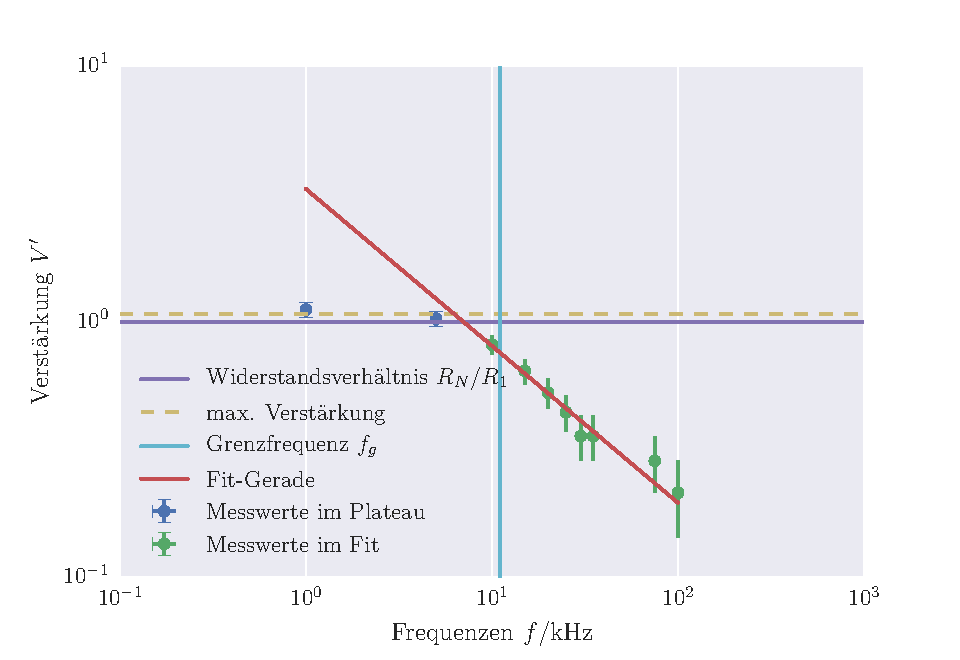
\includegraphics[scale=1]{../Grafiken/Gegengekoppelter_Verstaerker_1.pdf}
\caption{\label{fig:gegengekoppelter_verstaerker_1}}
\end{figure}
\FloatBarrier

\begin{table}[!h]
	\centering
	\begin{tabular}{ccc}
		\toprule
		Frequenz & Ausgangsspannung & Ausgangsspannung\\
		$f$/\si{\hertz} & $U_{A,\mathrm{int}}$/\si{\milli\volt} & $U_{A,\mathrm{diff}}$/\si{\milli\volt}\\
\midrule
		\num{100(1)} & \num{670(10)} & \num{140(10)}\\
		\num{200(2)} & \num{350(10)} & \num{240(10)}\\
		\num{300(3)} & \num{250(10)} & \num{350(10)}\\
		\num{400(4)} & \num{180(10)} & \num{450(10)}\\
		\num{500(5)} & \num{160(10)} & \num{550(10)}\\
		\num{600(6)} & \num{140(10)} & \num{640(10)}\\
		\num{700(7)} & \num{120(10)} & \num{740(10)}\\
		\num{800(8)} & \num{100(10)} & \num{840(10)}\\
		\num{900(9)} & \num{90(10)} & \num{920(10)}\\
		\num{1000(10)} & \num{80(10)} & \num{1040(10)}\\
		\bottomrule
	\end{tabular}
	\caption{ Messwerte der Frequenz der Eingangsspannung und der Ausgangsspannung für die Schaltungen eines Umkehrintegrators und -differentiators. \label{tab:integrator_differentiator}}
\end{table}

\FloatBarrier
\begin{figure}[!h]
\centering
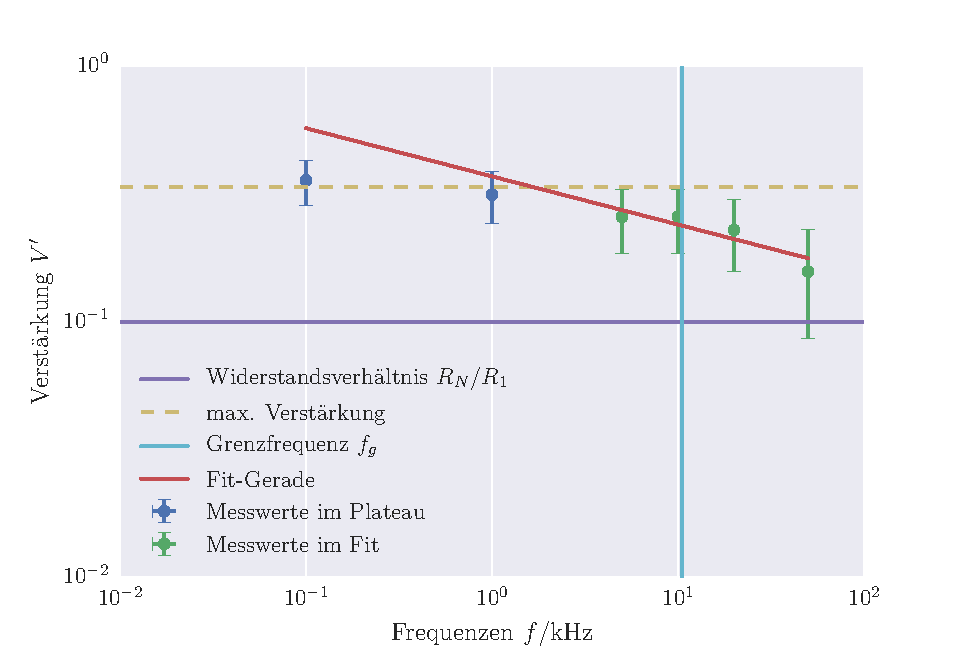
\includegraphics[scale=1]{../Grafiken/Gegengekoppelter_Verstaerker_2.pdf}
\caption{\label{fig:gegengekoppelter_verstaerker_2}}
\end{figure}
\FloatBarrier

\begin{table}[!h]
	\centering
	\begin{tabular}{ccc}
		\toprule
		Frequenz & Ausgangsspannung & Verstärkung\\
		$f$/\si{\kilo\hertz} & $U_{\mathrm{A}}$/\si{\milli\volt} & $V$\\
\midrule
		\num{0.0100(1)} & \num{37(5)} & \num{0.53(7)}\\
		\num{0.100(1)} & \num{35(5)} & \num{0.50(7)}\\
		\num{1.00(1)} & \num{38(5)} & \num{0.54(7)}\\
		\num{10.0(1)} & \num{32(5)} & \num{0.46(7)}\\
		\num{20.0(2)} & \num{30(5)} & \num{0.43(7)}\\
		\num{30.0(3)} & \num{25(5)} & \num{0.36(7)}\\
		\num{40.0(4)} & \num{19(5)} & \num{0.27(7)}\\
		\num{50.0(5)} & \num{19(5)} & \num{0.27(7)}\\
		\num{100(1)} & \num{16(5)} & \num{0.23(7)}\\
		\bottomrule
	\end{tabular}
	\caption{Messwerte der Frequenz und der Ausgangsspannung der dritten Schaltung eines gegengekoppelten Verstärkers.
            Zusätzlich ist die Verstärkung dieser Schaltung angegeben. \label{tab:gegengekoppelter_verstaerker_3}}
\end{table}

\FloatBarrier
\begin{figure}[!h]
\centering
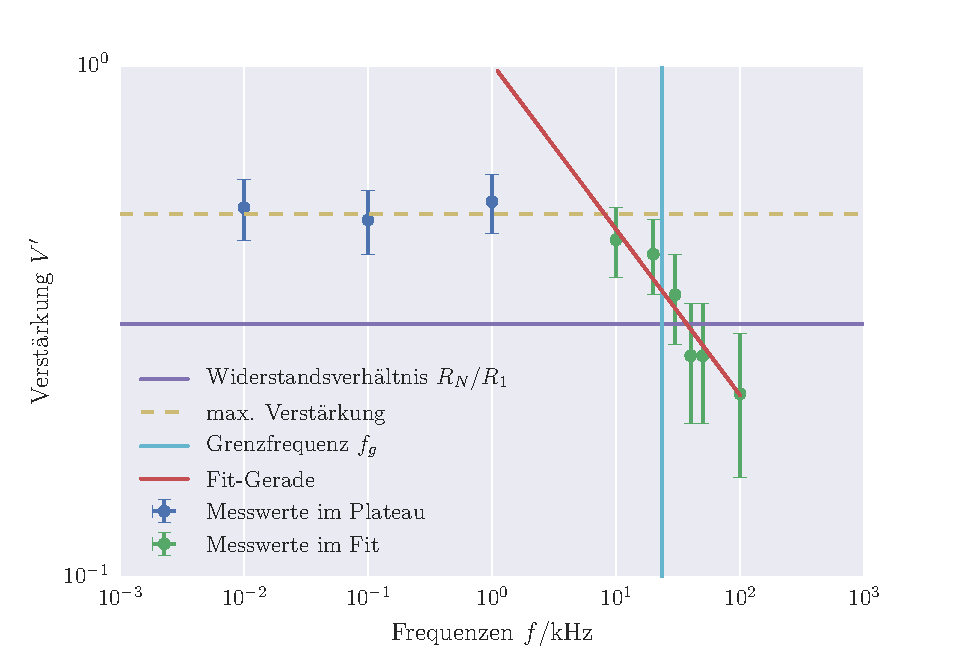
\includegraphics[scale=1]{../Grafiken/Gegengekoppelter_Verstaerker_3.pdf}
\caption{Doppellogarithmische Darstellung der Verstärkung der dritten gegengekoppelten Verstärkerschaltung in Abhängigkeit der Frequenz der Eingangsspannug. Zusätzlich wurden die Ausgleichsgerade
	durch die abfallenden Messwerte und eine senkrechte Gerade bei der Grenzfrequenz eingezeichnet. Ferner sind noch  zwei waagerechte Geraden dargestellt. Die eine markiert den Mittelwert der Messwerte im Plateau und die  andere
	den theoretischen Wert dieser Größe.\label{fig:gegengekoppelter_verstaerker_3}}
\end{figure}
\FloatBarrier

\begin{table}[!h]
	\centering
	\begin{tabular}{ccc}
		\toprule
		Frequenz & Ausgangsspannung & Verstärkung\\
		$f$/\si{\kilo\hertz} & $U_A$/\si{\milli\volt} & $V$\\
\midrule
		\num{0.100(1)} & \num{220(5)} & \num{3.14(8)}\\
		\num{1.00(1)} & \num{230(5)} & \num{3.29(9)}\\
		\num{5.00(5)} & \num{160(5)} & \num{2.29(8)}\\
		\num{10.0(1)} & \num{100(5)} & \num{1.43(7)}\\
		\num{20.0(2)} & \num{60(5)} & \num{0.86(7)}\\
		\num{30.0(3)} & \num{45(5)} & \num{0.64(7)}\\
		\num{50.0(5)} & \num{35(5)} & \num{0.50(7)}\\
		\num{100(1)} & \num{25(5)} & \num{0.36(7)}\\
		\bottomrule
	\end{tabular}
	\caption{Messwerte der Frequenz und der Ausgangsspannung der vierten Schaltung eines gegengekoppelten Verstärkers.
            Zusätzlich ist die Verstärkung dieser Schaltung angegeben. \label{tab:gegengekoppelter_verstaerker_4}}
\end{table}

\FloatBarrier
\begin{figure}[!h]
\centering
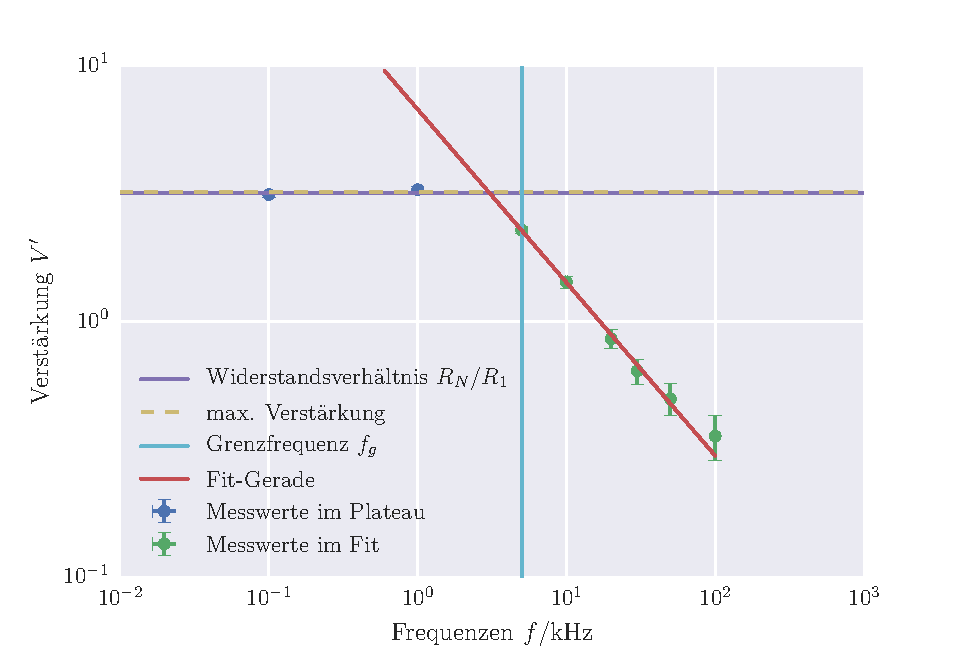
\includegraphics[scale=1]{../Grafiken/Gegengekoppelter_Verstaerker_4.pdf}
\caption{\label{fig:gegengekoppelter_verstaerker_4}}
\end{figure}
\FloatBarrier

\begin{table}[!h]
	\centering
	\begin{tabular}{ccc}
		\toprule
		Theoretische Verstärkung & Gemessene Verstärkung & relative Abweichung\\
		$V^{\prime}$ & $V^{\prime}_{\mathrm{max}}$ & $\Delta_{\mathrm{rel}} 
		V$/\si{\percent}\\
\midrule
		\num{1.000} & \num{1.071} & \num{7.143}\\
		\num{0.100} & \num{0.336} & \num{235.714}\\
		\num{0.312} & \num{0.514} & \num{64.571}\\
		\num{3.200} & \num{3.214} & \num{0.446}\\
		\bottomrule
	\end{tabular}
	\caption{ Vergleich der Werte der theoretischen Verstärkung der Schaltung, welche dem Verhältnis der verbauten 
Widerstände entspricht, mit dem Mittelwert der der gemessenen Verstärkungen vor dem linearen Abfall in doppellogarithmischer Darstellung. \label{tab:gegengekoppelter_verstaerker_max_verstaerkung}}
\end{table}

\begin{table}[!h]
	\centering
\begin{adjustbox}{width=1\textwidth}
	\begin{tabular}{ccccc}
		\toprule
		Steigung & $y$-Achsenabschnitt & Grenzfrequenz & Verstärkung-Bandbreite & Leerlaufverstärkung\\
		$a$ & $b$ & $f_{\mathrm{g}}$/\si{\kilo\hertz} & 
		$f_{\mathrm{g}}V^{\prime}_{\mathrm{max}}$/\si{\kilo\hertz} & $V$\\
\midrule
		\num{-0.61(4)} & \num{0.52(6)} & \num{11.025} & \num{11.813} & \num{-15.000}\\
		\num{-0.19(7)} & \num{-0.43(8)} & \num{10.562} & \num{3.546} & \num{-0.142}\\
		\num{-0.32(6)} & \num{0.00(8)} & \num{23.453} & \num{12.061} & \num{-0.796}\\
		\num{-0.68(2)} & \num{0.83(2)} & \num{5.013} & \num{16.112} & \num{-720.000}\\
		\bottomrule
	\end{tabular}
\end{adjustbox}
	\caption{ Parameter der Ausgleichskurven der abfallenden Verstärkung, sowie die Grenzfrequenz und das 
Verstärkung-Bandbreiten-Produkt für jeder der vier Schaltungen. Bezeichnet werden die Parameter mit Steigung und 
y-Achsenabschnitt, da die Parameter in doppellogarithmischer Darstellung diese Bedeutung haben. \label{tab:gegengekoppleter_verstaerker_parameter}}
\end{table}

\FloatBarrier

Es ist zu erkennen, dass für 
Widerstandsverhältnisse $ \geq 1$ der theoretische Wert gut mit dem gemittelten 
Wert übereinstimmt. Die relativen Abweichungen der Messwerte von den 
theoretischen Werten sind in einzeln in
\cref{tab:gegengekoppelter_verstaerker_max_verstaerkung} aufgeführt.
Bei den Widerstandsverhältnissen  $ < 1$ zeigt sich eine deutlich größere 
Abweichung der gemessenen Werte, welche aufgrund der doppellogarithmischen 
Darstellung jedoch größer zu seien scheint als diese in Wirklichkeit ist. 

Die Parameter der Ausgleichsrechnungen der Form
\begin{empheq}{equation}
V^{\prime}(f) = f^{a} \cdot 10^{b}  
\label{eq:fit}
\end{empheq}
der abfallenden Verstärkung sind zusammen mit der Grenzfrequenzen $f_{\mathrm{g}}$ und dem 
Verstärk\-ung-Bandbreiten-Produkten $f_{\mathrm{g}}V^{\prime}_{\mathrm{max}}$ 
in \cref{tab:gegengekoppleter_verstaerker_parameter} eingetragen.
Die Grenzfrequenzen wurden dabei nach
\begin{empheq}{align}
V^{\prime}(f_{\mathrm{g}}) &= \frac{V^{\prime}_{\mathrm{max}}}{\sqrt{2}} = f_{\mathrm{g}}^{a} \cdot 10^{b}\\
\Leftrightarrow f_{\mathrm{g}} &= \del{\frac{V^{\prime}_{\mathrm{max}}}{\sqrt{2}\cdot 10^b}}^{\dfrac{1}{a}}
\end{empheq}


bestimmt. 
In doppellogarithmischer Darstellung haben die Parameter $a$ und $b$ die 
Bedeutung der Steigung respektive des $y$-Achsenabschnittes der Geraden.
Des Weiteren wurde auch die Leerlaufspannung $V$ abgeschätzt, indem
\cref{eq:leerlauf_verstaerkung} zu  
\begin{empheq}{equation}
	V = \frac{V^{\prime}R_{\mathrm{N}}}{R_{\mathrm{N}} -V^{\prime}R_{1}}
\end{empheq}
umgeformt wurde. Die entsprechenden Werte wurden ebenfalls in 
\cref{tab:gegengekoppleter_verstaerker_parameter} eingetragen.


Der Frequenzgang der Verstärkerschaltung lässt sich mit dem in 
\cref{fig:ersatzschaltbild} dargestellten Ersatzschaltbild eines idealen 
Operationsverstärkers 
mit nachgeschaltetem Tiefpass erklären.

\FloatBarrier
\begin{figure}[!h]
\centering
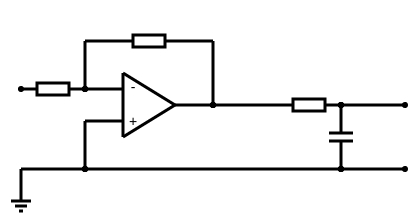
\includegraphics[scale=1]{../Grafiken/Ersatzschaltbild.jpg}
\caption{Ersatzschaltbild eines realen Operationsverstärkers 
	in dem dieser durch einen idealen Operationsverstärker und einen 
	nachgeschalteten Tiefpass ersetzt wird. Der Tiefpass beschreibt dabei 
	interne Widerstände und Kapazitäten des realen Operationsverstärkers.
	\label{fig:ersatzschaltbild}}
\end{figure}
\FloatBarrier

Die Messwerte des Frequenzgangs der Phasenbeziehung zwischen Ein- und 
Ausgangsspannung sind in \cref{tab:gegengekoppelter_verstaerker_phase}
aufgelistet und in \cref{fig:gegengekoppelter_verstaerker_phase} graphisch 
dargestellt. In dem Frequenzbereich in dem der gegengekoppelte Verstärker die Verstärkung
$V^{\prime}_{\mathrm{max}}$ liefert, ist zu erkennen, dass die Ausgangsspannung gegenüber der 
Eingangsspannung \SI{180}{\degree} phasenverschoben. Mit zunehmender Frequenz nimmt diese 
Phasenverschiebung ab auch dieses Verhalten ist dem eines Tiefpasses ähnlich.  



\begin{table}[!h]
	\centering
	\begin{tabular}{cc}
		\toprule
		Frequenz & Phase\\
		$f$/\si{\kilo\hertz} & $\Delta \phi$/\si{\degree}\\
\midrule
		\num{0.100(1)} & \num{175(5)}\\
		\num{0.200(2)} & \num{170(5)}\\
		\num{0.300(3)} & \num{168(5)}\\
		\num{0.400(4)} & \num{168(5)}\\
		\num{0.500(5)} & \num{165(5)}\\
		\num{1.00(1)} & \num{162(5)}\\
		\num{2.00(2)} & \num{150(5)}\\
		\num{3.00(3)} & \num{140(5)}\\
		\num{4.00(4)} & \num{130(5)}\\
		\num{5.00(5)} & \num{125(5)}\\
		\num{10.0(1)} & \num{110(5)}\\
		\num{20.0(2)} & \num{90(5)}\\
		\bottomrule
	\end{tabular}
	\caption{Messwerte der Frequenz und der Phase zwischen Eingangs- und Ausgangsspannung der vierten Schaltung 
eines gegengekoppelten Verstärkers. \label{tab:gegengekoppelter_verstaerker_phase}}
\end{table}

\FloatBarrier
\begin{figure}[!h]
\centering
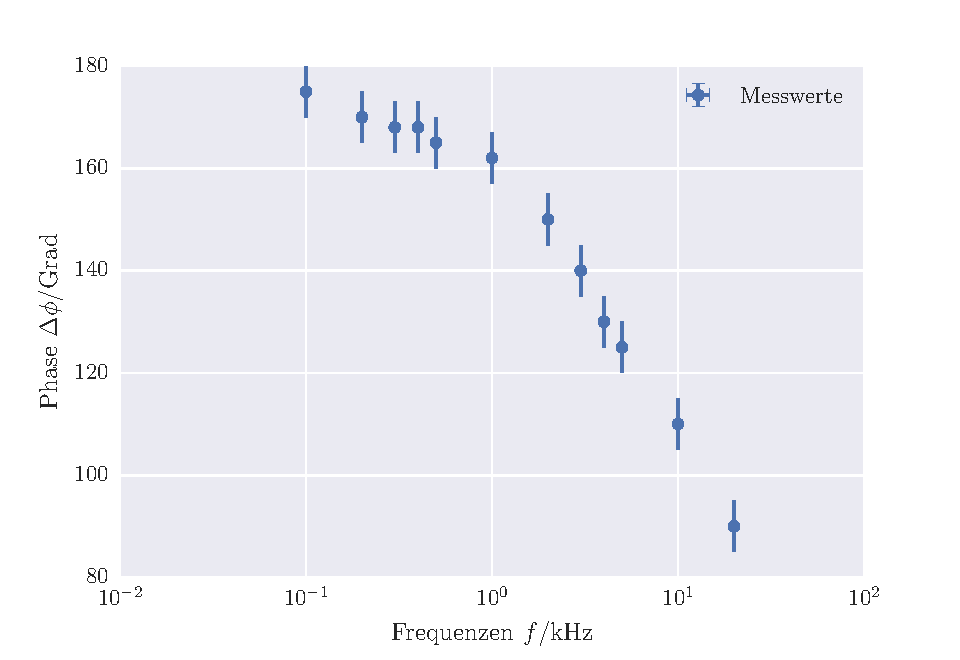
\includegraphics[scale=1]{../Grafiken/Gegengekoppelter_Verstaerker_Phase.pdf}
\caption{\label{fig:gegengekoppelter_verstaerker_phase}}
\end{figure}
\FloatBarrier



\subsection{Amperemeter mit geringem Eingangswiderstand}

Die am Amperemeter aufgenommenen Messwerte sind in \cref{tab:amperemeter_1}
einzusehen, wobei zusätzlich die theoretische Ausgangsspannung 
$U_{A,\mathrm{theo}}$ durch Einsetzen des Stroms $I~=~\sfrac{U_{g}}{R_{V}}$ 
in \cref{eq:amperemeter_strom} nach
\begin{empheq}{equation}
	U_\text{A}= \frac{U_{\mathrm{g}}}{R_{\mathrm{V}}} R_\text{N}
\end{empheq}
berechnet wurde. Des Weiteren wurde die relative Abweichung der gemessenen Ausgangsspannung $U_A$ von 
dieser bestimmt. Der Eingangswiderstand $r_{e}$ ergibt sich für diese Schaltung wie angegeben nach
\begin{empheq}{equation}
	r_{\mathrm{e}} = \frac{U_{\mathrm{e}}}{I} = \frac{U_{\mathrm{E}}R_{\mathrm{V}}}{U_{\mathrm{g}}}
\end{empheq}
Die Lehrlaufverstärkung $V$ der verwendeten Schaltung ergibt sich durch Umformung von 
\cref{eq:eingangswiderstand} nach
\begin{empheq}{equation}
	V = \frac{R_{\mathrm{N}}}{r_{\mathrm{e}}}=\frac{R_{\mathrm{N}}}{R_{\mathrm{V}}} 
	\frac{U_{\mathrm{g}}}{U_{\mathrm{E}}}.
\end{empheq}
Für den Aufbau der Schaltung wurden die Widerstände
$R_{\mathrm{V}} = \SI{100(1)}{\ohm}$ und\\ $R_{\mathrm{N}} = \SI{10.0(1)}{\kilo\ohm}$ 
verwendet.
In  \cref{tab:amperemeter_2} sind die berechneten Werte für den
Innenwiderstand $r_e$ und die Leerlaufverstärkung $V$ angegeben. 
Die graphischen Darstellungen der dieser beiden Größen in Abhängigkeit der
Frequenz ist in 
%\cref{fig:amperemeter_eingangswiderstand} und 
\cref{fig:amperemeter_leerlaufverstaerkung_eingangswiderstand} gezeigt.

\begin{table}[!h]
	\centering
	\begin{adjustbox}{width=1\textwidth}
	\begin{tabular}{cccccc}
		\toprule
		Frequenz & Generatorspannung & Eingangsspannung & Ausgangsspannung & Ausgangsspannung & Ausgangsspannung\\
		$f$/\si{\kilo\hertz} & $U_{\mathrm{g}}$/\si{\milli\volt} & $U_{\mathrm{E}}$/\si{\milli\volt} & $U_{\mathrm{A}}$/\si{\volt} & $U_{\mathrm{A},\mathrm{theo}}$/\si{\volt} & $\Delta_{\mathrm{rel}}U_{\mathrm{A}}$/\si{\percent}\\
\midrule
		\num{100(1)} & \num{0.209(1)} & \num{0.023(2)} & \num{20.0(1)} & \num{20.9(3)} & \num{4(2)}\\
		\num{200(2)} & \num{0.207(1)} & \num{0.023(2)} & \num{20.0(1)} & \num{20.7(3)} & \num{3(2)}\\
		\num{500(5)} & \num{0.207(1)} & \num{0.030(2)} & \num{20.0(1)} & \num{20.7(3)} & \num{3(2)}\\
		\num{750(8)} & \num{0.207(1)} & \num{0.035(2)} & \num{20.0(1)} & \num{20.7(3)} & \num{3(2)}\\
		\num{1000(10)} & \num{0.207(1)} & \num{0.040(2)} & \num{20.0(1)} & \num{20.7(3)} & \num{3(2)}\\
		\num{1500(15)} & \num{0.207(1)} & \num{0.050(2)} & \num{19.0(1)} & \num{20.7(3)} & \num{8(2)}\\
		\num{2000(20)} & \num{0.207(1)} & \num{0.060(2)} & \num{19.0(1)} & \num{20.7(3)} & \num{8(2)}\\
		\num{2500(25)} & \num{0.207(1)} & \num{0.075(2)} & \num{19.5(1)} & \num{20.7(3)} & \num{6(2)}\\
		\num{3000(30)} & \num{0.207(1)} & \num{0.085(2)} & \num{19.5(1)} & \num{20.7(3)} & \num{6(2)}\\
		\num{3500(35)} & \num{0.207(1)} & \num{0.095(2)} & \num{19.5(1)} & \num{20.7(3)} & \num{6(2)}\\
		\num{4000(40)} & \num{0.207(1)} & \num{0.105(2)} & \num{18.0(1)} & \num{20.7(3)} & \num{14(2)}\\
		\num{4500(45)} & \num{0.207(1)} & \num{0.110(2)} & \num{18.7(1)} & \num{20.7(3)} & \num{10(2)}\\
		\num{5000(50)} & \num{0.207(1)} & \num{0.125(2)} & \num{18.3(1)} & \num{20.7(3)} & \num{13(2)}\\
		\num{5500(55)} & \num{0.207(1)} & \num{0.140(2)} & \num{18.0(1)} & \num{20.7(3)} & \num{14(2)}\\
		\num{6000(60)} & \num{0.207(1)} & \num{0.150(2)} & \num{17.5(1)} & \num{20.7(3)} & \num{18(2)}\\
		\num{6500(65)} & \num{0.207(1)} & \num{0.160(2)} & \num{17.3(1)} & \num{20.7(3)} & \num{19(2)}\\
		\num{7000(70)} & \num{0.207(1)} & \num{0.170(2)} & \num{16.9(1)} & \num{20.7(3)} & \num{22(2)}\\
		\num{7500(75)} & \num{0.207(1)} & \num{0.185(2)} & \num{16.5(1)} & \num{20.7(3)} & \num{25(2)}\\
		\num{8500(85)} & \num{0.207(1)} & \num{0.195(2)} & \num{16.3(1)} & \num{20.7(3)} & \num{26(2)}\\
		\num{9000(90)} & \num{0.207(1)} & \num{0.200(2)} & \num{15.7(1)} & \num{20.7(3)} & \num{31(2)}\\
		\num{10000(100)} & \num{0.207(1)} & \num{0.215(2)} & \num{14.7(1)} & \num{20.7(3)} & \num{40(2)}\\
		\bottomrule
	\end{tabular}
\end{adjustbox}
	\caption{ Messwerte der Frequenz der Eingangsspannung, der Generator-, der Eingangs- und Ausgangsspannung
der Ampermeterschaltung. Zusätzlich ist die theoretische Ausgangsspannung und der realtive Unterschied zwischen dieser
und der gemessenen angegeben. \label{tab:amperemeter_1}}
	
\end{table}


\begin{table}[!h]
	\centering
	\begin{tabular}{cccc}
		\toprule
		Frequenz & Strom & Eingangswiderstad & Leerlaufverstärkung\\
		$f$/\si{\kilo\hertz} & $I$/\si{\ampere} & $r_{\mathrm{e}}$/\si{\ohm} & $V$\\
\midrule
		\num{100(1)} & \num{0.00209(2)} & \num{11(1)} & \num{908(80)}\\
		\num{200(2)} & \num{0.00207(2)} & \num{11(1)} & \num{899(79)}\\
		\num{500(5)} & \num{0.00207(2)} & \num{14(1)} & \num{690(47)}\\
		\num{750(8)} & \num{0.00207(2)} & \num{16(1)} & \num{591(35)}\\
		\num{1000(10)} & \num{0.00207(2)} & \num{19(1)} & \num{517(27)}\\
		\num{1500(15)} & \num{0.00207(2)} & \num{24(1)} & \num{413(18)}\\
		\num{2000(20)} & \num{0.00207(2)} & \num{28(1)} & \num{345(13)}\\
		\num{2500(25)} & \num{0.00207(2)} & \num{36(1)} & \num{276(8)}\\
		\num{3000(30)} & \num{0.00207(2)} & \num{41(1)} & \num{243(7)}\\
		\num{3500(35)} & \num{0.00207(2)} & \num{45(1)} & \num{217(6)}\\
		\num{4000(40)} & \num{0.00207(2)} & \num{50(1)} & \num{197(5)}\\
		\num{4500(45)} & \num{0.00207(2)} & \num{53(1)} & \num{188(4)}\\
		\num{5000(50)} & \num{0.00207(2)} & \num{60(1)} & \num{165(4)}\\
		\num{5500(55)} & \num{0.00207(2)} & \num{67(1)} & \num{147(3)}\\
		\num{6000(60)} & \num{0.00207(2)} & \num{72(1)} & \num{138(3)}\\
		\num{6500(65)} & \num{0.00207(2)} & \num{77(1)} & \num{129(2)}\\
		\num{7000(70)} & \num{0.00207(2)} & \num{82(1)} & \num{121(2)}\\
		\num{7500(75)} & \num{0.00207(2)} & \num{89(1)} & \num{111(2)}\\
		\num{8500(85)} & \num{0.00207(2)} & \num{94(1)} & \num{106(2)}\\
		\num{9000(90)} & \num{0.00207(2)} & \num{96(1)} & \num{103(2)}\\
		\num{10000(100)} & \num{0.00207(2)} & \num{103(1)} & \num{96(2)}\\
		\bottomrule
	\end{tabular}
	\caption{ Aus den gemessenen Spannungen der Amperemeterschaltung berechnete Werte des Stroms und des Eingangswiderstands
sowie die aus letzterem berechneten Werte der Leerlaufverstärkung. \label{tab:amperemeter_2}}
\end{table}


%\FloatBarrier
\begin{figure}[!h]
\centering
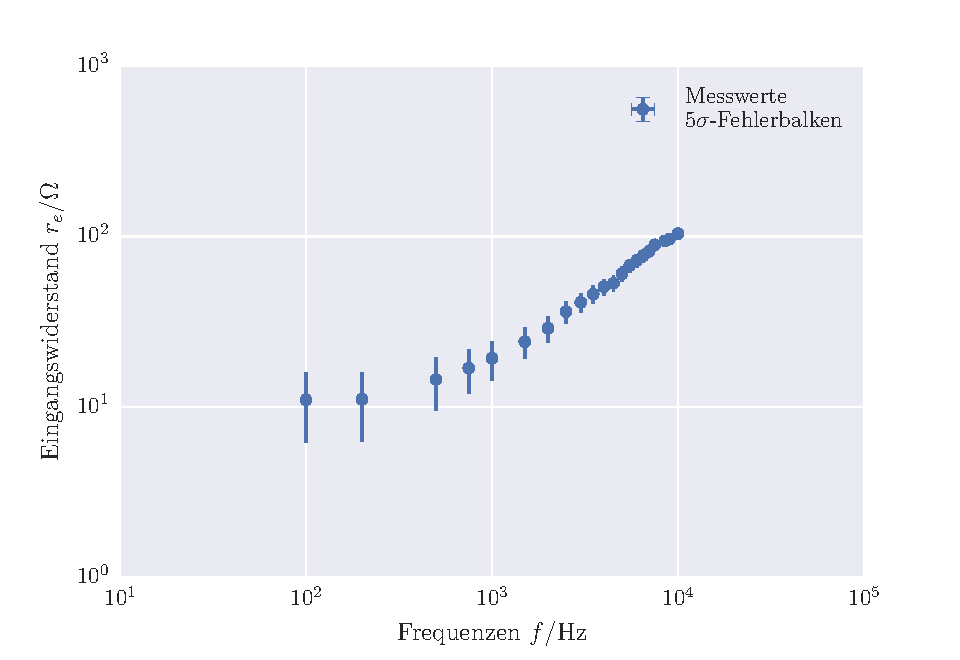
\includegraphics[scale=1]{../Grafiken/Amperemeter_Eingangswiderstand.pdf}
\caption{Doppellogarithmische Darstellung des Eingangswiderstands der Amperemeterschaltung
	in Abhängigkeit der Frequenz. \label{fig:amperemeter_eingangswiderstand}}
\end{figure}
\FloatBarrier
%\FloatBarrier
\begin{figure}[!h]
\centering
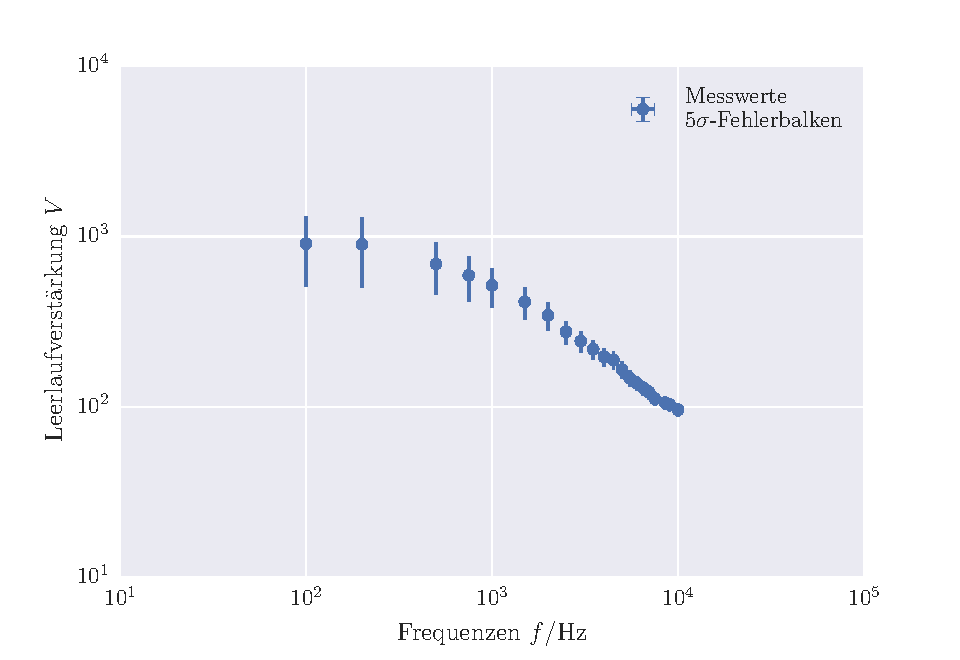
\includegraphics[scale=1]{../Grafiken/Amperemeter_Leerlaufverstaerkung.pdf}
\caption{Doppellogarithmische Darstellung des Leerlaufverstärkung der Amperemeterschaltung
	in Abhängigkeit der Frequenz.  \label{fig:amperemeter_leerlaufverstaerkung}}
\end{figure}
\FloatBarrier
\FloatBarrier
\begin{figure}[!h]
\centering
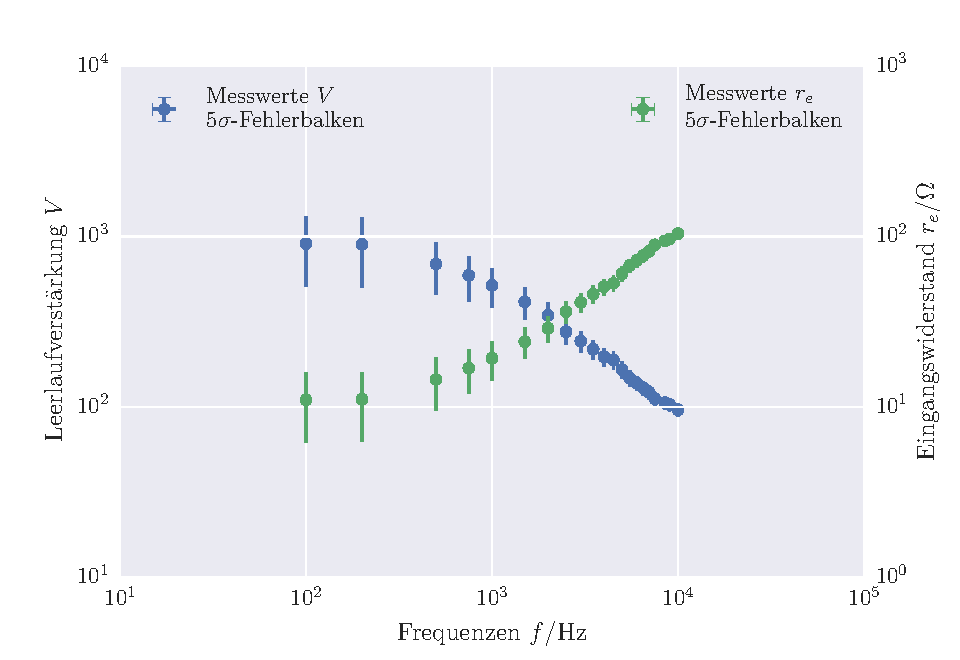
\includegraphics[scale=1]{../Grafiken/Amperemeter_Leerlaufverstaerkung_Eingangswiderstand.pdf}
\caption{Doppellogarithmische Darstellung des Leerlaufverstärkung $V$ (linke Skala, blaue) und des
	Eingangswiderstandes $r_{\mathrm{e}}$
	(rechte Skala, grün) der Amperemeterschaltung in Abhängigkeit der
	Frequenz.\label{fig:amperemeter_leerlaufverstaerkung_eingangswiderstand}}
\end{figure}
\FloatBarrier

\subsection{Integrator- und Differentiatorschaltung}

Die für Integrator- und Diffentiatorschaltungen aufgenommenen Messwerte
befinden sich in \cref{tab:integrator_differentiator}.
Die doppellogaritmische Darstellung der Frequenzabhängigkeit der 
Ausgangsspannung des Integrators ist in \cref{fig:integrator_frequenz}
und die des Differentiators in \cref{fig:differentiator_frequenz} gezeigt.
Zusätzlich zu den Messwerte ist auf das Ergebnis einer Ausgleichsrechnung nach
\cref{eq:fit} abgebildet. Die Parameter der Ausgleichskurven sind:
\begin{empheq}{alignat=2}
	a_{\mathrm{int}} &= \num{-0.91(1)} \qquad& a_{\mathrm{diff}} = 
	\num{0.90(1)}\\
	b_{\mathrm{int}} &= \num{4.64(2)} \qquad& b_{\mathrm{diff}} = 
	\num{0.31(3)}
\end{empheq}
%integrator
%Steigung a           -0.906547929601287 +/- 0.01060464728719671
%y-Achsenabschnitt b  4.637839462233714 +/- 0.023588320273295587
%differentiator
%Steigung a           0.8994746172449467 +/- 0.01152732378072151
%y-Achsenabschnitt b  0.31231762902616494 +/- 0.0330777456740357

In den Abbildungen \ref{fig:integrator_oszilloskop_sinus} --  
\ref{fig:integrator_oszilloskop_rechteck} und 
\ref{fig:differentiator_oszilloskop_sinus} --  
\ref{fig:differentiator_oszilloskop_rechteck} sind jeweils die 
Ausgangsspannungen des Integrators respektive des Differentiators
für die drei Eingangsspannungen Sinus, Dreieck und Rechteck dargestellt.


\begin{table}[!h]
	\centering
	\begin{tabular}{ccc}
		\toprule
		Frequenz & Ausgangsspannung & Ausgangsspannung\\
		$f$/\si{\hertz} & $U_{A,\mathrm{int}}$/\si{\milli\volt} & $U_{A,\mathrm{diff}}$/\si{\milli\volt}\\
\midrule
		\num{100(1)} & \num{670(10)} & \num{140(10)}\\
		\num{200(2)} & \num{350(10)} & \num{240(10)}\\
		\num{300(3)} & \num{250(10)} & \num{350(10)}\\
		\num{400(4)} & \num{180(10)} & \num{450(10)}\\
		\num{500(5)} & \num{160(10)} & \num{550(10)}\\
		\num{600(6)} & \num{140(10)} & \num{640(10)}\\
		\num{700(7)} & \num{120(10)} & \num{740(10)}\\
		\num{800(8)} & \num{100(10)} & \num{840(10)}\\
		\num{900(9)} & \num{90(10)} & \num{920(10)}\\
		\num{1000(10)} & \num{80(10)} & \num{1040(10)}\\
		\bottomrule
	\end{tabular}
	\caption{ Messwerte der Frequenz der Eingangsspannung und der Ausgangsspannung für die Schaltungen eines Umkehrintegrators und -differentiators. \label{tab:integrator_differentiator}}
\end{table}


\FloatBarrier
\begin{figure}[!h]
\centering
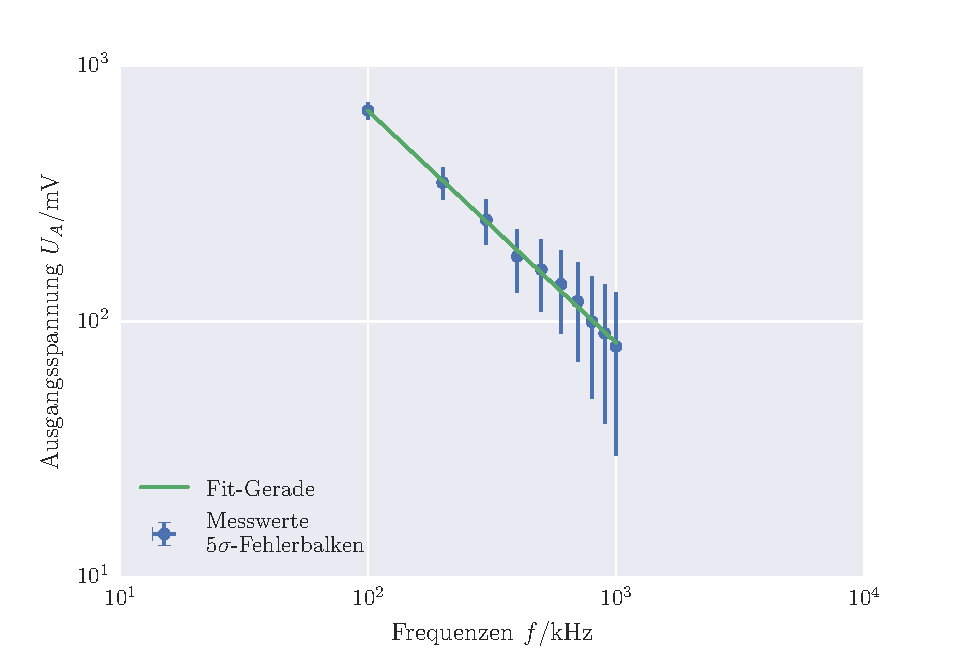
\includegraphics[scale=1]{../Grafiken/Integrator_Frequenz.pdf}
\caption{\label{fig:integrator_frequenz}}
\end{figure}
\FloatBarrier
\FloatBarrier
\begin{figure}[!h]
\centering
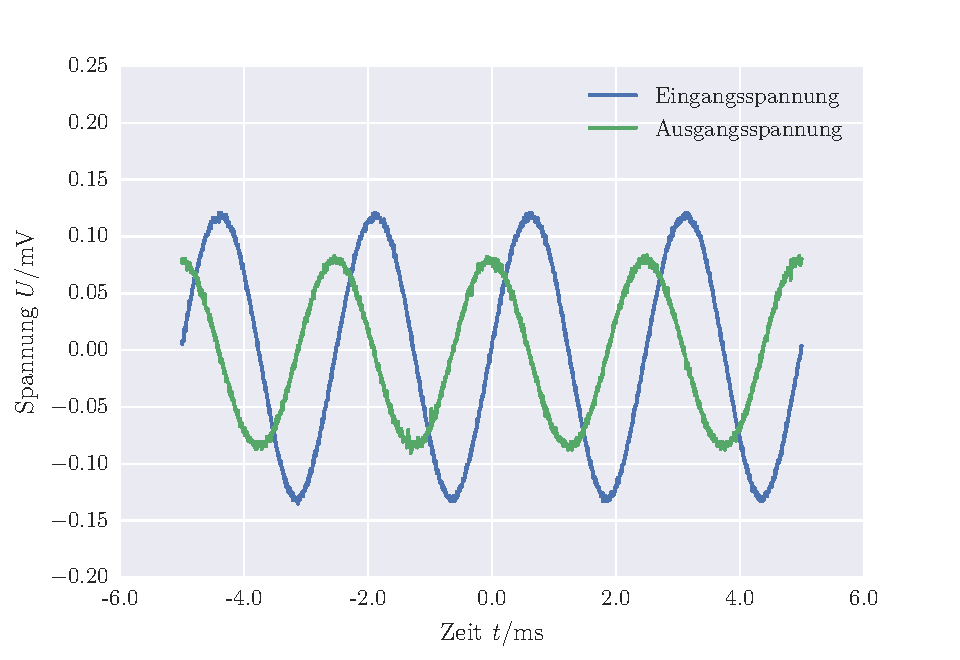
\includegraphics[scale=1]{../Grafiken/Integrator_Oszilloskop_Sinus.pdf}
\caption{Vom Oszilloskop aufgenommene Ein- und Ausgangsspannungen der Integratorschaltung. Auf dem Eingang
	liegt hier eine Sinusspannung. \label{fig:integrator_oszilloskop_sinus}}
\end{figure}
\FloatBarrier
\FloatBarrier
\begin{figure}[!h]
\centering
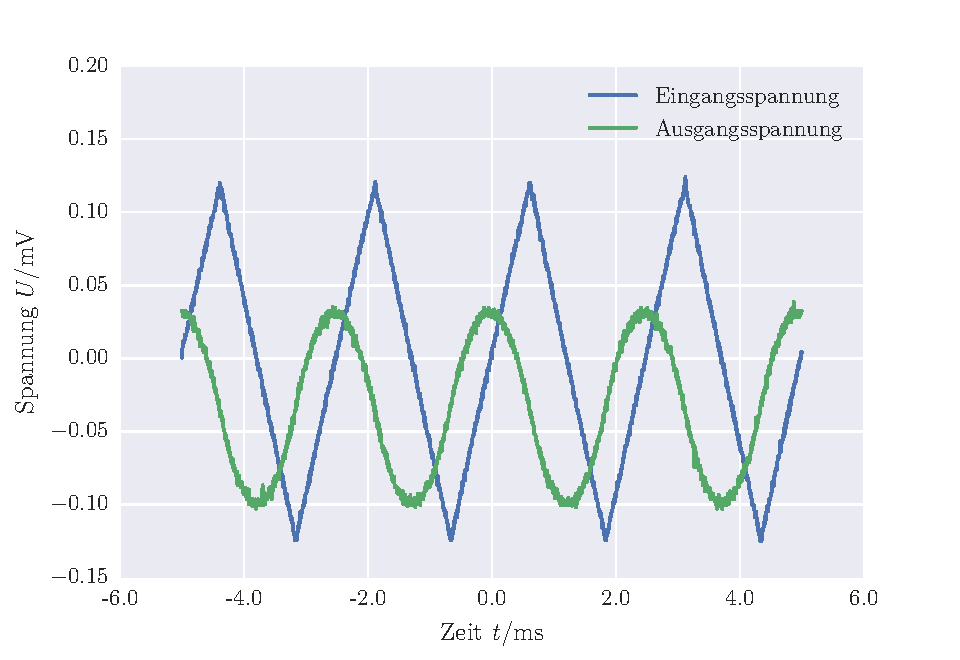
\includegraphics[scale=0.75]{../Grafiken/Integrator_Oszilloskop_Dreieck.pdf}
\caption{Vom Oszilloskop aufgenommene Ein- und Ausgangsspannungen der Integratorschaltung. Auf dem Eingang
	liegt hier eine Dreicksspannung. Die Ausgangsspannung in Parabelform entspricht dem theoretisch
	zu erwartendem Verlauf (periodische Abfolge nach oben respektive nach unten geöffneter 
	Parabeln).\label{fig:integrator_oszilloskop_dreieck}}
\end{figure}
\FloatBarrier
\FloatBarrier
\begin{figure}[!h]
\centering
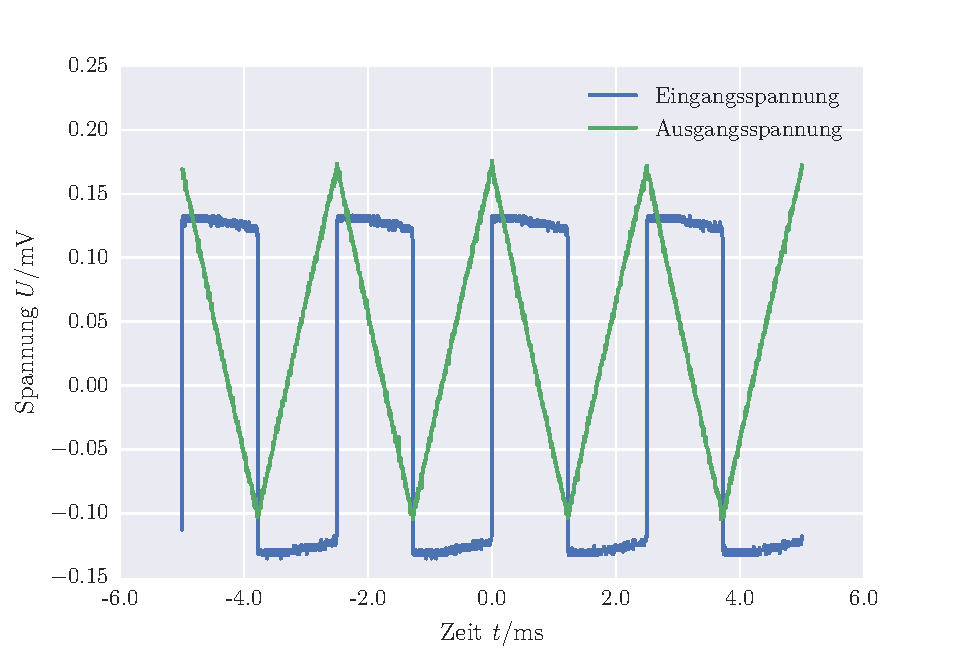
\includegraphics[scale=0.75]{../Grafiken/Integrator_Oszilloskop_Rechteck.pdf}
\caption{Vom Oszilloskop aufgenommene Ein- und Ausgangsspannungen der Integratorschaltung. Auf dem Eingang
	liegt hier eine Rechteckspannung.  Die Ausgangsspannung in Form einer Dreieckspannung entspricht dem theoretisch
	zu erwartendem Verlauf.\label{fig:integrator_oszilloskop_rechteck}}
\end{figure}
\FloatBarrier
\FloatBarrier
\begin{figure}[!h]
\centering
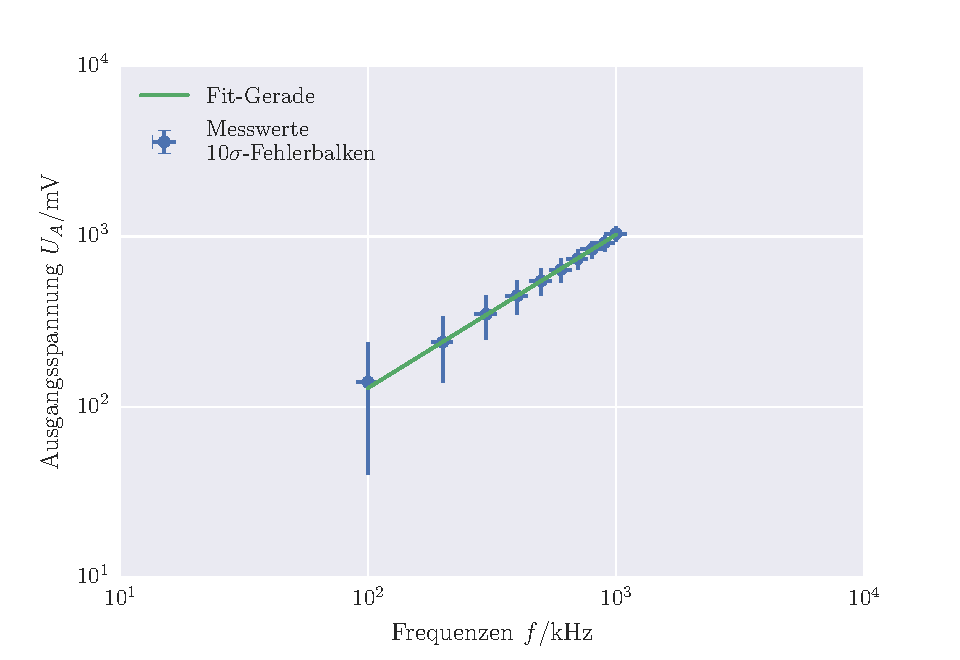
\includegraphics[scale=1]{../Grafiken/Differentiator_Frequenz.pdf}
\caption{\label{fig:differentiator_frequenz}}
\end{figure}
\FloatBarrier
\FloatBarrier
\begin{figure}[!h]
\centering
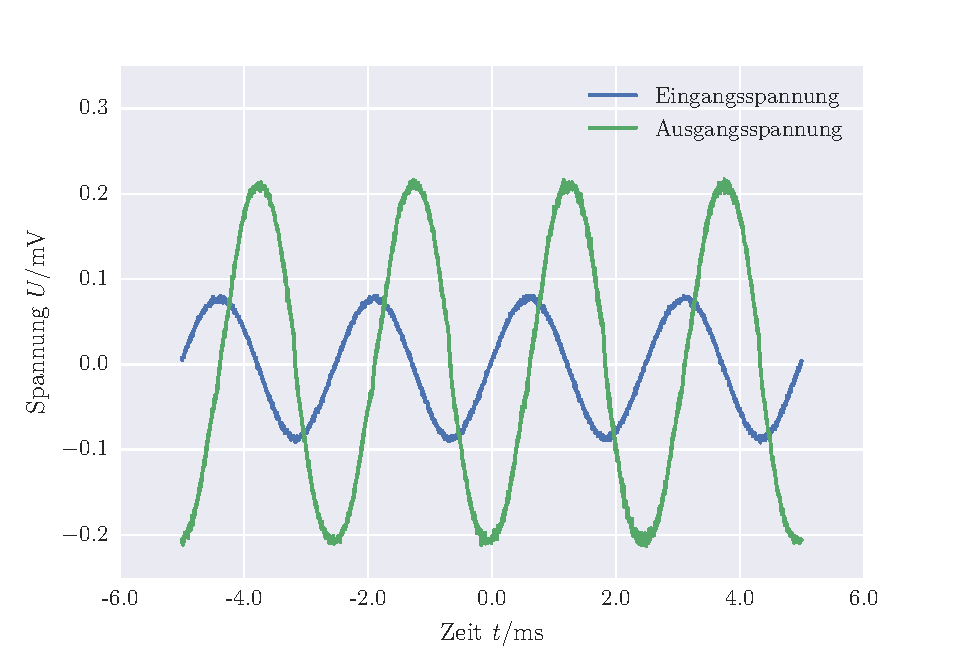
\includegraphics[scale=0.75]{../Grafiken/Differentiator_Oszilloskop_Sinus.pdf}
\caption{Vom Oszilloskop aufgenommene Ein- und Ausgangsspannungen der Differentiatorschaltung. Auf dem Eingang
	liegt hier eine Sinusspannung.\label{fig:differentiator_oszilloskop_sinus}}
\end{figure}
\FloatBarrier
\FloatBarrier
\begin{figure}[!h]
\centering
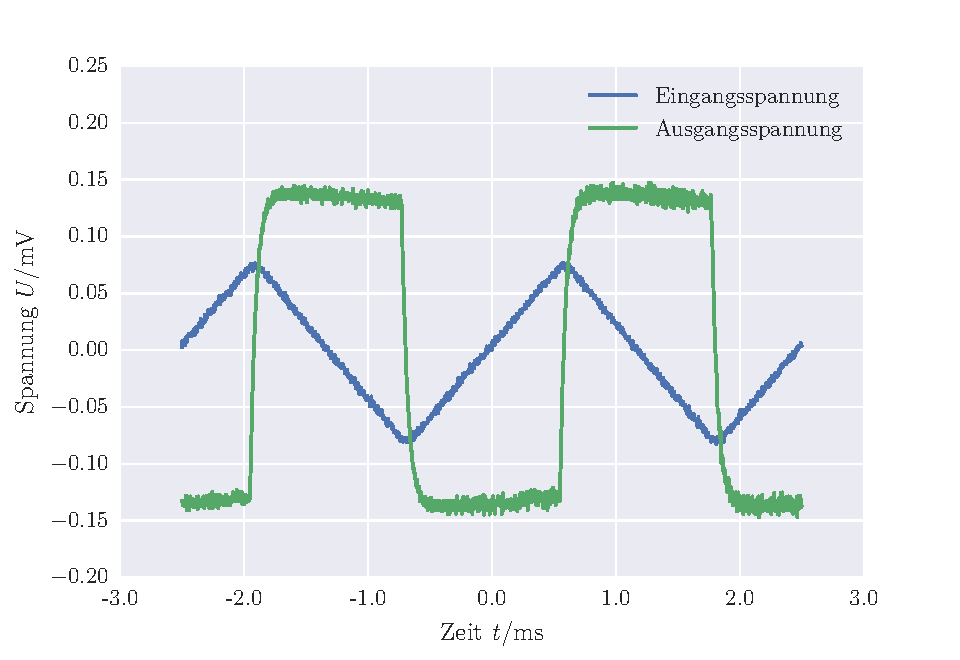
\includegraphics[scale=1]{../Grafiken/Differentiator_Oszilloskop_Dreieck.pdf}
\caption{\label{fig:differentiator_oszilloskop_dreieck}}
\end{figure}
\FloatBarrier
\FloatBarrier
\begin{figure}[!h]
\centering
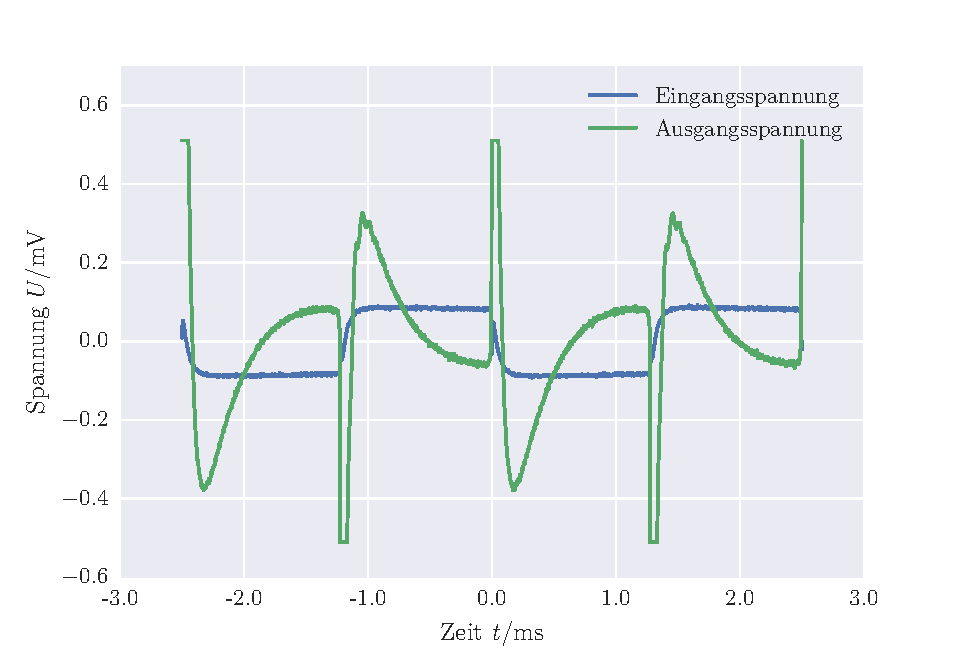
\includegraphics[scale=0.75]{../Grafiken/Differentiator_Oszilloskop_Rechteck.pdf}
\caption{Vom Oszilloskop aufgenommene Ein- und Ausgangsspannungen der Differentiatorschaltung. Auf dem Eingang
	liegt hier eine Rechteckspannung. Die Ausgangsspannung in Form schmalen hohen Peaks entspricht in etwa dem 
	theoretisch zu erwartendem Verlauf eines Delta-Kamms.\label{fig:differentiator_oszilloskop_rechteck}}
\end{figure}
\FloatBarrier

\subsection{Schmitt-Trigger}

Die für den Aufbau der Schmitt-Trigger-Schaltung verwendeten Bauteile
und aufgenommenen Messwerte hatten die folgenden Größen:
\begin{empheq}{align*}
	R_1 &= \input{../Ergebnisse/schmitt_trigger_R1.txt}\\
	R_{\mathrm{P}} &= \input{../Ergebnisse/schmitt_trigger_Rp.txt}\\
	U_{\mathrm{K}} &= \input{../Ergebnisse/schmitt_trigger_UK.txt}\\
	U_{\mathrm{A}} &= \input{../Ergebnisse/schmitt_trigger_UA.txt}\\
	U_{\mathrm{B}} &= \frac{U_{\mathrm{A}}}{2}
\end{empheq}
Die gemessene Kippspannung des Schmitt-Triggers $U_{\mathrm{K}}$ weicht damit von dem 
nach \cref{eq:kippspannug} theoretisch bestimmten Wert $U_{\mathrm{K},\mathrm{theo}} = 
\SI{0.66(1)}{\volt}$ in etwa um \SI{68}{\percent} ab.


\subsection{Funktionsgenerator}

Für den Aufbau der Schaltung wurden die folgenden Bauteile verwendet:
\begin{empheq}{alignat*=2}
R &= \SI{560(6)}{\ohm}  \qquad& C = \SI{1.00(1)}{\micro\farad}\\
R_1 &= \SI{1.00(1)}{\kilo\ohm}\qquad& R_0 = \SI{32.0(3)}{\kilo\ohm}\\
R_{\mathrm{P}} &= \SI{100(1)}{\kilo\ohm}\qquad& R^{\prime}_0 = \SI{10.0(1)}{\kilo\ohm}
\end{empheq}
Die Schaltung wurde um die zwei Widerstände $R_0$ und $R^{\prime}_0$ ergänzt,
die sich so ergebende Schaltung ist in \cref{fig:funktionsgenerator_real} 
dargestellt.

\FloatBarrier
\begin{figure}[!h]
\centering
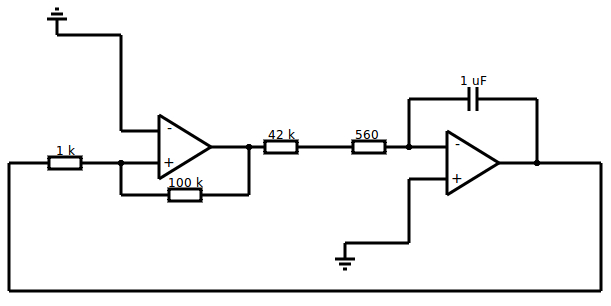
\includegraphics[scale=0.6]{../Grafiken/Funktionsgenerator_real.jpg}
\caption{Die verwendete Schaltung eines 
Funktionsgenerators. Es wurden zwei  zusätzliche Widerstände in Reihe 
(dargestellt ist nur die Summe beider Widerstände) geschaltet, um 
die Eingangspannung des zweiten Operationsverstärkers zu verringern.
\label{fig:funktionsgenerator_real}}
\end{figure}
\FloatBarrier

Die Ausgangsspannungen des Funktionsgenerators, die mit Hilfe des Oszilloskops
aufgenommen wurden sind in \cref{fig:funktionsgenerator} dargestellt.
Die  Frequenz und Amplitude der Rechteck- respektive Dreiecksspannung 
ergaben sich zu:
\begin{empheq}{align*}
f_{\mathrm{R}} &= \SI{570(1)}{\hertz} \qquad& f_{\mathrm{D}} = 
\SI{570(1)}{\hertz}\\
U_{\mathrm{A},\mathrm{R}} &= \SI{0.235(1)}{\volt} \qquad& U_{\mathrm{A},\mathrm{D}} = 
\SI{0.165(1)}{\volt}
\end{empheq}
Die theoretische Frequenz ergibt sich nach \cref{eq:funktionsgenerator_frequenz}
mit der Korrektur durch die beiden Widerstände $R_0$ und $R^{\prime}_0$ zu
\begin{empheq}{equation}
	f_{\mathrm{\mathrm{R},\mathrm{theo}}} = 
	f_{\mathrm{\mathrm{D},\mathrm{theo}}} =  
	\SI{587(11)}{\hertz}.
\end{empheq}
Die Scheitelwerte der Spannungen ergeben sich mit der Betriebsspannung $\SI{15.0(1)}{\volt}$ ebenfalls nach Korrektur
durch $R_0$ und $R^{\prime}_0$ für die Rechteckspannung $U_{\mathrm{A},\mathrm{R},\mathrm{theo}}$
aus \cref{eq:funktionsgenerator_rechteck} respektive \cref{eq:funktionsgenerator_dreieck} zu
\begin{empheq}{align}
U_{\mathrm{A},\mathrm{R},\mathrm{theo}} &= \SI{0.197(3)}{\volt}\\
U_{\mathrm{A},\mathrm{D},\mathrm{theo}} &=  \SI{0.150(2)}{\volt}.
\end{empheq}



\FloatBarrier
\begin{figure}[!h]
\centering
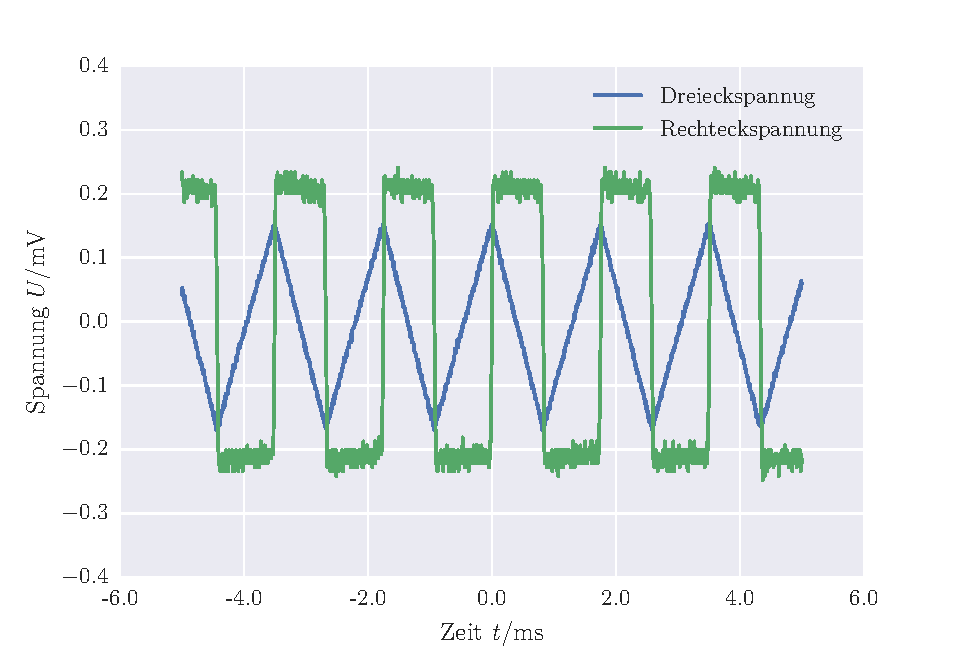
\includegraphics[scale=1]{../Grafiken/Funktionsgenerator.pdf}
\caption{Vom Oszilloskop aufgenommene Rechteck- und Dreiecksspannung der Funktionsgeneratorschaltung.\label{fig:funktionsgenerator}}
\end{figure}
\FloatBarrier



